\chapter{Preliminaries}

Topological Data Analysis is a wide topic, where results from all Mathematical branches are put together in order to compute topological invariants among real world data. A basic understanding of algebra, analysis, and geometry is required to approach the theoretical results that underpin the core theory, which establishes the necessary structures and their stability. Therefore, to establish a common foundation and unify the diverse notations and procedures found in the literature, this chapter introduces the key definitions and basic results needed for the rest of the thesis.

Section \ref{sec:preliminaries-homology} makes a 
brief recall of simplicial homology in order to define persistent homology modules. Section \ref{sec:preliminaries-modules} then introduces persistence modules, the algebraic tool used to study the structure of persistence homology groups. Section \ref{sec:preliminaries-barcodes} introduces a tool to summarize the data from the persistence homology groups, the barcodes. With this summary it is possible to compute how homologically different are two datasets, or how different are two filtrations among the same data. To make this measure, the interleaving and bottleneck distance are introduced. The first one measures distances between persistence modules, while the latter one measures distance between the barcodes of those modules. One key aspect of them, is that they are actually equivalent, as its later proved in Chapter \ref{chap:interleaving-stability}.

A visual way of presenting barcodes is through persistence diagrams. Both barcodes and persistence diagrams are equivalent ways of presenting the homological features of data. To give a different perspective about how to measure distances between persistence diagrams, Section \ref{sec:preliminaries-wp-persistance} introduces the Wasserstein distance and redefines the bottleneck distance as a particular case.

Finally, Section \ref{sec:preliminaries-hausdorff} recalls the Hausdorff distance to measure distance between subsets of metric spaces, and generalices it presenting the Gromov-Hausdorff distance, which allows to measure distances between sets located in different metric spaces. This will be useful to delimit bottleneck distance in order to proof its stability.


Section \ref{sec:preliminaries-homology} primarily follows \cite{wang}. Sections \ref{sec:preliminaries-modules} and \ref{sec:preliminaries-barcodes} are based on the presentation at \cite{polterovich}. Section \ref{sec:preliminaries-wp-persistance} takes the definitions given at \cite{bubenik2} and Section \ref{sec:preliminaries-hausdorff} follows \cite{burago}.

\section{Persistent homology} \label{sec:preliminaries-homology}

In most Algebraic Topology introductory texts, homology is first presented in the form of homology groups (see \cite{munkres}, \cite{hatcher}). We are going to generalize homology groups to homology $R$-modules based on the notes by Wang \cite{wang}. This makes possible to take coefficients over an arbitrary commutative ring $ R $ and will lead us to introduce persistent homology and the persistence modules. Lets star recalling what an $R$-module is, to be followed by a brief presentation of simplicial homology.

\begin{definition}[$R$-module, Definition IV.1.1.1 \cite{hungerford}]
    Let $ R $ be a commutative ring. An {\bf $R$-module } is an abelian group $ (M, +) $ with an operation $ \cdot \colon R \times M \to M $ such that for all $ r, s \in R $ and for all $ x, y \in M $,
    \begin{enumerate}
    \renewcommand{\labelenumi}{(\roman{enumi})}
        \item $ (rs) \cdot x = r (s \cdot x) $,
        \item $ (r + s) \cdot x = r \cdot x + s \cdot x $,
        \item $ r \cdot (x + y) = r \cdot x + r \cdot y $.
    \end{enumerate}
    If $ R $ has a multiplicative identity $ 1 $, then $ M $ is said to be a {\bf unitary $R$-module} and 
    \begin{enumerate}
    \renewcommand{\labelenumi}{(\roman{enumi})}
        \setcounter{enumi}{3}
        \item $1 \cdot x = x $.
    \end{enumerate}
    If $ R $ is a division ring, that is, a ring with identity where every non cero element is a unit, then 
    a unitary $R$-module is called a {\bf left $R$-vector space}. Note that in this case, $R$ is in fact a field. Also note that, when we take $ R = (\Z, +, \cdot) $, a $\Z$ module is actually an abelian group.
\end{definition}

\begin{definition}[Affinely independent touple]
    A $ (k+1)$-tuple of points $ (x_0, \dots, x_k) $ in $ \R^n $, where each 
    $ x_i \in \R^n $ is said to be {\bf affinely independent} if the set of vectors $ \{ x_j - x_0 \mid 1 \leq j \leq k \}$ is linearly independent.
\end{definition}

\begin{definition}[$k$-simplex]
    A {\bf $k$-simplex} is an ordered $(k+1)$-tuple of affinely independent points $\sigma = (x_0, \dots, x_k)$. The {\bf vertices} of $\sigma$ are the points of the set $ V = \{ x_0, \dots, x_k \} $. Every simplex $\sigma$ induces a total ordering $\preccurlyeq_{\sigma}$ on its set of vertices $V$, where if $p \leq q$, then $x_p \preccurlyeq_{\sigma} x_q$ in $V$. For $m \leq n$, an $(m + 1)$-tuple $(y_0, \dots, y_m)$, where each $y_j \in V$ and if $j \leq k$, then $y_j \preccurlyeq_{\sigma} y_k$, is called an {\bf $m$-face} of $\sigma$.
\end{definition}

\begin{definition}[Abstract simplicial complex]
    An {\bf abstract simplicial complex} $K $ is a finite collection of simplices such that for every face of a simplex in $ K $ is also a simplex in $ K $.
\end{definition}

\begin{definition}[Simplicial $k$-chain]
    Let $R$ be a commutative ring with additive identity $0 $ and multiplicative identity $1$ and let $K$ be a simplicial complex. A {\bf simplicial $k$-chain} is a formal sum of $k$-simplices,
    \begin{equation}
        \sum_{i=1}^{N} r_i \sigma_i,
    \end{equation}
    such that $r_i \in R$ and $\sigma_i \in K $.
\end{definition}

Note that that set of simplicial $k$-chains with formal addition over $R$ form a $R$-module. Denote that $R$-module as $K_k$.

\begin{definition}[Boundary map]
    Let $ K $ be a simplicial complex, and let $ K_k $ and $ K_{k-1} $ be two $ R$-modules from $ K $. For every $k$-simplex $\sigma =  (x_0, \dots, x_k) \in K $, the {\bf boundary} map $ \partial_k \colon K_k \to K_{k-1} $ is defined as
    \begin{equation}
        \partial_k(\sigma) = \sum_{i=0}^{k} (-1)^i (x_0, \dots, \hat x_i, \dots, x_k),
    \end{equation}
    where $ (x_0, \dots, \hat x_i, \dots, x_k) $ denotes the $(k-1)$-face of $\sigma $ obtained by removing the vertex $x_i$.
\end{definition}

As the boundary map can be extends linearly to arbitrary $k$-chains, it forms an $R$-module homomorphism $\partial_k \colon K_k \to K_{k-1}$.

\begin{definition}[Chain complex]
    A {\bf chain complex} $(K, d)$ is a sequence of $R$-modules $ A_k $ with boundary maps $ d_k \colon A_k \to A_{k-1} $, such that the composition $ d_{k-1} \circ d_k = 0 $ for all $k \leq 0$.
\end{definition}

\begin{lemma}[Lemma 2.1, \cite{hatcher}]
    The collection of $R$-modules $K_k$ connected by boundary maps $\partial_k$ forms a chain complex $(K, \partial)$.
\end{lemma}
\begin{proof}
    We just need to prove that for every $k$-simplex $\sigma = (x_0, \dots, x_k) $ for $ k \geq 1 $, we get $ \partial_{k-1} \circ \partial_k (\sigma) = 0$. By linearity of the boundary map, we can just compute
    \begin{align}
        \partial_{k-1} \circ \partial_k (\sigma) = & \sum_{i=0}^{k} (-1)^i \partial_{k-1} (x_0, \dots, \hat x_i, \dots, x_k) \\
        = & \sum_{j < i} (-1)^i (-1)^j (x_0, \dots, \hat x_j, \dots, \hat x_j, \dots, x_k) \\
        & + \sum_{j > i} (-1)^i (-1)^{j-1} (x_0, \dots, \hat x_i, \dots, \hat x_j, \dots, x_k).
    \end{align}
    The last two sums vanish as when changing $ i $ and $j $ positions in the second, it becomes the negative of the first.
\end{proof}

\begin{corolary}
    The boundary maps $\partial_k$ satisfy that for every $k \leq 0$, $\im \partial_{k+1} \subseteq \ker \partial_k $.
\end{corolary}
\begin{proof}
    If there is some $k$-simplex $\sigma \in \im(\partial)$ then there exists some $(k+1)$-simplex $\tau$ such that $ \partial_{k+1} \tau = \sigma $. Hence, as $ \partial_k \circ \partial_k+1 = 0 $,we have that $ \partial_k(\partial_{k+1} \tau) = \partial_k \sigma = 0 $ and $ \sigma \in \ker(\partial_k) $.
\end{proof}

\begin{definition}[Homology module]
    Let $K $ be a simplicial complex. The {\bf $k$-th homology module} of $K$ is the $R$-module given by
    \begin{equation}
        H_k(K) \coloneq \frac{\ker \partial_k}{\im \partial_{k+1}}.
    \end{equation} 
\end{definition}

Homology can be extended to every topological space, not just those that are triangulable by introducing singular homology (see \cite{munkres}[Chapter 4]). However, in this work, we will restrict ourselves to simplicial homology. This choice is motivated by the nature of the data typically encountered in topological data analysis. The spaces involved are usually "sufficiently nice" and therefore triangulable. Moreover, real-world data intended for computational analysis is finite by nature, and hence, triangulable. Furthermore, simplicial homology of a finite simplicial complex $K$ is computable (see \cite{munkres}[Theorem 11.5]) what makes it a prefect tool for computational studies.

\begin{definition}[Filtration]
    Let $ K $ be a simplicial complex and let $ T $ be a complete ordered index set. A {\bf filtration} of $ K $ is a nested sequence of subcomplexes $ F_i K $, $ i \in T $, such that for every $ i \in T $, 
    \begin{equation}
        F_i \subseteq F_{i+1}.
    \end{equation}
    We will denote the {\bf inclusion simplicial maps} by $ g_i \colon F_i \hookrightarrow F_{i+1} K $.
\end{definition}

Filtrations are a natural way of obtaining simplicial complexes from datasets, as it is posible to set the first element of the filtration to be the points in the datasets, and then join in various steps each of the point to form a simplicial complex that connects every point by simplices of different dimensions. Naturally, depending on the procedure we follow we could get quite different filtration for one same dataset.

\begin{example} \label{ex:filtration}
    Figure \ref{fig:filtration} depicts a posible filtration of a simplicial complex $K$ in four steps. It starts with four 0-simplices and one 1-simplex at $ F_0 K $ and ads components until it has six $0$-simplices, six 1-simplices and one 2-simplex at $ F_3 K $.
        \begin{figure}[H]
        \centering
        \begin{subfigure}[b]{0.45\linewidth}
            \centering
            \begin{tikzpicture}[line cap=round, line join=round, x=1cm, y=1cm]
                \clip (-0.5, 0) rectangle (5, 3.5);
                \coordinate (a) at (0.21, 0.14);
                \coordinate (b) at (0.62, 2.82);
                \coordinate (c) at (2.01, 1.32);
                \coordinate (d) at (4.23, 2.23);
                \draw (c) -- (d);
                \foreach \point/\pos in {a/above left, b/above left, c/below right, d/above right}
                    \draw[fill=black] (\point) circle (1pt) node[\pos] {$\point$};
            \end{tikzpicture}
            \caption*{$F_0 K$}
        \end{subfigure}
        \hfill
        \begin{subfigure}[b]{0.45\linewidth}
            \centering
            \begin{tikzpicture}[line cap=round, line join=round, x=1cm, y=1cm]
                \clip (-0.5, 0) rectangle (5, 3.5);
                \coordinate (a) at (0.21, 0.14);
                \coordinate (b) at (0.62, 2.82);
                \coordinate (c) at (2.01, 1.32);
                \coordinate (d) at (4.23, 2.23);
                \draw (c) -- (d) -- (b) -- cycle;
                \foreach \point/\pos in {a/above left, b/above left, c/below right, d/above right}
                    \draw[fill=black] (\point) circle (1pt) node[\pos] {$\point$};
            \end{tikzpicture}
            \caption*{$F_1 K$}
        \end{subfigure}

        \vspace{0.5cm} % Add vertical space between rows

        \begin{subfigure}[b]{0.45\linewidth}
            \centering
            \begin{tikzpicture}[line cap=round, line join=round, x=1cm, y=1cm]
                \clip (-0.5, 0) rectangle (5, 3.5);
                \coordinate (a) at (0.21, 0.14);
                \coordinate (b) at (0.62, 2.82);
                \coordinate (c) at (2.01, 1.32);
                \coordinate (d) at (4.23, 2.23);
                \coordinate (e) at (4.64, 0.91);
                \coordinate (f) at (2.78, 0.63);
                \draw (a) -- (b) -- (c) -- cycle;
                \draw (c) -- (d) -- (b);
                \foreach \point/\pos in {a/above left, b/above left, c/below right, d/above right, e/below right, f/below}
                    \draw[fill=black] (\point) circle (1pt) node[\pos] {$\point$};
            \end{tikzpicture}
            \caption*{$F_2 K$}
        \end{subfigure}
        \hfill
        \begin{subfigure}[b]{0.45\linewidth}
            \centering
            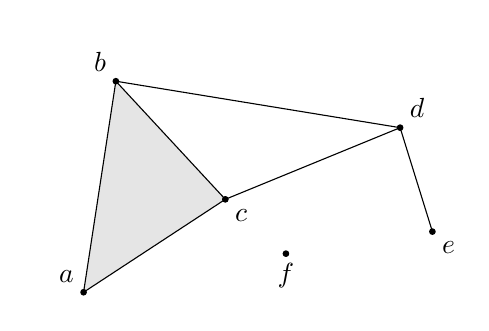
\begin{tikzpicture}[line cap=round, line join=round, x=1cm, y=1cm]
                \clip (-0.5, 0) rectangle (5, 3.5);
                \coordinate (a) at (0.21, 0.14);
                \coordinate (b) at (0.62, 2.82);
                \coordinate (c) at (2.01, 1.32);
                \coordinate (d) at (4.23, 2.23);
                \coordinate (e) at (4.64, 0.91);
                \coordinate (f) at (2.78, 0.63);
                \fill[fill=black, fill opacity=0.1] (a) -- (b) -- (c) -- cycle;
                \draw (a) -- (b) -- (c) -- cycle;
                \draw (c) -- (d) -- (b);
                \draw (d) -- (e);
                \foreach \point/\pos in {a/above left, b/above left, c/below right, d/above right, e/below right, f/below}
                    \draw[fill=black] (\point) circle (1pt) node[\pos] {$\point$};
            \end{tikzpicture}
            \caption*{$F_3 K$}
        \end{subfigure}
        \caption{Four step filtration of a simplicial complex $K$.}
        \label{fig:filtration}
    \end{figure}
\end{example}

Considering a filtration of a simplicial complex, we can compute the homology groups at each step of the filtration. Hence, for each $ k \geq 0 $, there are induced linear maps $ H_kg_i \colon H_k(F_iK) \to H_k(F_{i+1}K) $ that fit together into a sequence of vector spaces
\begin{equation}
\begin{tikzcd}
    H_k(F_0K) \arrow[r, "H_kg_0"] & H_k(F_1K) \arrow[r, "H_kg_1"] & \cdots \arrow[r, "H_kg_{n-2}"] & H_k(F_{n-1}K) \arrow[r, "H_kg_{n-1}"] & H_k(F_nK).
\end{tikzcd}
\end{equation}
As homology is functorial, when we consider the inclusion map formed by the composition of several others, the induced map at homology level also becomes a composition of the corresponding maps. That is, for any pair $ i \leq j $ of indices, where $ i, j = 1, \dots, n $, the map induced on homology by the inclusion map $ g_{i \leq j} \colon F_i K \hookrightarrow F_j K $, is given by the composition
\begin{equation}
    H_k g_{i \leq j} = H_k g_{j-1} \circ H_k g_{j-2} \circ \cdots \circ H_k g_{i+1} \circ H_k g_i.
\end{equation}

Such maps $ H_k g_{i \leq j} $ give really relevant information about our data, as they permit us to relate the $k$-th homology groups of every subcomplex $ F_i K $ that appear in a filtration of $ K $.

Now if $ X $ is a triangulable topological space, and $ f \colon X \to T $, we can extend the concept of filtration to be attained to $ X $. For clarity, fix $ T = \R $. Hence, for each $ a \in \R $, the pre image of the interval $(-\infty, a] $ by $ f $ is some subspace $ X_a $ of $ X $. That is,
\begin{equation}
    f^{-1}((-\infty, a]) = X_a.
\end{equation}
As $ X $ is triangulable, we will look for functions that satisfy that each $ X_a $ is triangulable too. An therefore we can compute its homology module.

\begin{definition}[Homological critical value] \label{def:critical-value}
    Let $ X $ be a topological space and let $ f\colon X \to \R $. A {\bf homological critical value} of $ f $ is a number $ a \in \R $ such that there exists $k \in \Z$ such that for all 
    $ \e > 0 $, the morphism $ H_k(f^{-1}(-\infty, a - \e]) \to H_k(f_{-1}(-\infty, a + \e]) $ is not an isomorphism.
\end{definition}

\begin{definition}[Tame function] \label{def:tame-function}
    A function $ f\colon X \to \R $ is said to be {\bf tame} if it has a finite number of homological critical values, and for all $ z \in \Z $, and for all $ a \in \R $, $ \dim F_a < \infty $.
\end{definition}

\begin{example}[Piecewise linear functions]
    The first example of tame functions, and the one we will most make use of, are piecewise linear functions.
\end{example}
\begin{proof}
    To prove that piecewise linear functions are tame, we need to verify the two conditions in Definition \ref{def:tame-function}:

    First we will check that piecewise linear functions have a finite number of homological critical values. A piecewise linear function $ f \colon X \to \mathbb{R} $ is defined by its values on the vertices of a simplicial complex and is linearly interpolated on the simplices. The function $ f $ can only change the homology of its sublevel sets at the values it takes on the vertices. Since a simplicial complex has finitely many vertices, $ f $ has finitely many such values. These are the only candidates for homological critical values. Thus, $ f $ has finitely many homological critical values.

    Now, we need to check that every sublevel sets has finite-dimensional homology. For any $ a \in \R $, the sublevel set $ f^{-1}(-\infty, a] $ is a subcomplex of the simplicial complex $ X $ (or a subset thereof). Because $ f $ is linear on each simplex, $ f^{-1}(-\infty, a] $ consists of all simplices where $ f \leq a $ on all vertices. The homology groups of a finite simplicial complex are finitely generated (and thus finite-dimensional when using field coefficients). Hence, $ \dim H_k(f^{-1}(-\infty, a]) < \infty $ for all $ k \in \Z $.
\end{proof}

\begin{example}[Morse functions]
    A real function defined over a differential manifold, $ f\colon M \to \R $ it is said to be a {\bf Morse function} if it has no degenerate analytical critical points. Recall that analytical critical points are those were the differential of $ f $ vanishes. A critical point $ p \in \R $ is degenerate if the Hessian matrix determinant vanish.

    By how Morse functions are defined, if they are taken over a compact manifold, then Morse functions are tame.
\end{example}

\begin{example}[Non-tame function]
    Of course, not every function is tame. A classic counterexample comes from the topologist's sine curve $ f: [0, 1] \in \R $ defined as
    \begin{equation}
        f(x) = \begin{cases}
            \sin(\frac{1}{x}) &\text{ if } x \neq 0, \\
            0 &\text{ if } x = 0,
        \end{cases}
    \end{equation}
    Note that the interval $ [0, 1] $ is isomorphic to a simplicial complex formed by one 1-simplex and two 0-simplices. As $ x $ tends to $ 0 $, $ \sin(\frac{1}{x}) $ oscillates between 1 and -1. Hence, each local extremum $ a $ of $ \sin(\frac{1}{x}) $ introduces a change in the topology of the sublevel sets $ f^{-1}(-\infty, a] $, creating infinitely many homological critical values.
\end{example}

\begin{definition}[Persistent homology module] \label{def:persistent-homology}
    Let $X$ be a triangulable topological space and let $ f \colon X \to \R $. For every fixed $ k \in \Z $, we denote
    \begin{equation}
        F_x \coloneq H_k(f^{-1}(-\infty, x]),
    \end{equation}
    and for every $ x \leq y $, we denote the induced inclusion map from $ X_x $ to $ X_y $ as
    \begin{equation}
        f_x^y \colon F_x \to F_y.
    \end{equation}
    The {\bf persistent homology module} associated to $ x $ and $ y $ is the subspace of $X_y$ given by 
    \begin{equation}
        F_x^y \coloneq \im f_x^y.
    \end{equation}
    The {\bf persistent Betti numbers} are defined as
    \begin{equation}
        \beta_x^y \coloneq \dim(F_x^y).
    \end{equation}
\end{definition}

\begin{example} \label{ex:persistent groups}
    We can compute persistent homology modules at each step of the filtration of Example \ref{ex:filtration}. For simplicity, We will fix the $R$-module homology, taking $R = \Z $, to compute classic group homology. Also note that for every $ k \neq 0, 1 $, homology groups will be the trivial ones, as there are no posible chain complexes of dimensions different from $ 0, 1 $ or $ 2 $. Recall that $0$-dimensional homology measures the number of path components of a space, and that $1$-dimensional homology counts the number of $1$-dimensional ``holes'' (see \cite{nina}[Section 3]).
    
    Hence for each step of the filtration $ F_i K $ we have:
    \begin{align}
        H_0(F_0 K) &= \Z^3,  & H_1(F_0 K) &= \{1\}, \\
        H_0(F_1 K) &= \Z^2,  & H_1(F_1 K) &= \Z, \\
        H_0(F_2 K) &= \Z^3,  & H_1(F_2 K) &= \Z^2, \\
        H_0(F_3 K) &= \Z^2,  & H_1(F_3 K) &= \Z.
    \end{align}
    Note that as this particular filtration is discrete, and there is not any isomorphism in each of the changes, every $ i = 0, 1, 2, 3 $ is a critical point both for $ k = 1 $ and for $ k = 2 $.
\end{example}

\section{Persistence modules and interleaving distance} \label{sec:preliminaries-modules}

To enable a more rigorous and structured study, we introduce the category of persistence modules along with their morphisms. This categorical framework provides the foundation for analyzing the stability and structure of persistent homology.

\begin{definition}[Persistence module]
    Let $\F$ be a field and let $T$ be a totally ordered set. Let $ V = \{V_t\}_{t \in T} $ be a collection of $F$-vector spaces. A $T$-indexed {\bf persistence module} is a pair $ (V, \pi) $ such that $ \pi = \{ \pi_{s \leq t} \} $ is a collection of linear maps $ \pi_{s \leq t}\colon V_s \rightarrow V_t $ that verifies that for all $ r, s, t \in T $,
    \begin{equation}
        \pi_{r \leq s} \circ \pi_{s \leq t} = \pi_{r \leq t}.
    \end{equation}
\end{definition}

\begin{definition}[Morphism between persistence modules]
    Let $T$ be a totally ordered set. Let $ (V, \pi), (W, \theta) $ be two persistence modules. A {\bf morphism} between persistence modules $ p \colon (V, \pi) \to (W, \theta) $ is a family of linear maps $ p_t \colon V_t \to W_t $ such that for all $ s \leq t $ the following diagram commutes:
    $$
    \begin{tikzcd}
        V_s \arrow[r, "\pi_{s \leq t}"] \arrow[d, "p_s"'] & V_t \arrow[d, "p_t"] \\
        W_s \arrow[r, "\theta_{s \leq t}"']               & W_t
    \end{tikzcd}
    $$
    If a morphism $ i $ verifies that for all $ t \in T $, $ i_t \colon V_t \to V_t $ is the identity, then $ i $ is the {\bf identity morphism}. If there exists two morphisms $ p \colon (V, \pi) \to (W, \theta) $ and $ q \colon (W, \theta) \to (V, \pi) $ such that the compositions $ p \circ q $ and $ q \circ p $ are both the identity morphism, then $ p $ and $ q $ are {\bf isomorphisms} of persistence modules. In this case, $ (V, \pi) $ and $ (W, \theta) $ are said to be {\bf isomorphic} persistence modules.
\end{definition}

For now on, to simplify notation, we will limit our totally ordered set to be the real numbers, $ T = \R $. Also, when there is no possible confusion, we might denote the persistence module $ (V, \pi) $ by just is collection of vector spaces $ V $. 

This section defines a distance between persistence modules that will allow us to differentiate how far are two modules from each other.

\begin{definition}[Persistence module shift]
    Let $ (V, \pi) $ be a persistence module and let $ \delta \in \R $. The {\bf $\delta$-shift} of $ (V, \pi) $ is the persistence module $ (V_\delta, \pi_\delta) $ defined by taking
    \begin{align}
        (V_\delta)_t &\coloneq V_{t+\delta}, \quad & (\pi_\delta)_{s\leq t} &\coloneq \pi_{s+\delta \leq t+\delta}.
    \end{align}
\end{definition}

\begin{proposition}[Exercise 1.2.3, \cite{polterovich}] \label{prop:shift-morphism}
    Let $ \delta > 0 $. Let $(V, \pi), (V_\delta, \pi_\delta) $ be a persistence module and its shift. The map $ \phi_\delta \colon (V, \pi) \to (V_\delta, \pi_\delta) $, defined as
    \begin{equation}
        \phi_\delta (V_t) \coloneq \pi_{t \leq t + \delta}(V_t) = V_{t+\delta},
    \end{equation}
    is a persistence module morphism.
\end{proposition}
\begin{proof}
    As $ \delta > 0 $, then $ t \leq t+\delta $. Hence
    \begin{align}
        \phi_\delta \circ \pi_{t \leq t+\delta} (V_t) &= \phi_\delta (V_{t+\delta}) = V_{t+\delta+\delta} = V_{t+2 \delta}, \\
        \pi_{t+\delta \leq t+2\delta} \circ \phi_\delta (V_t) &= \pi_{t+\delta \leq t+2\delta}(V_{t+\delta}) = V_{t+2 \delta}.
    \end{align}
\end{proof}

\begin{definition}[Shift morphism]
    The persistence module morphism $ \phi_\delta $ defined as in Proposition \ref{prop:shift-morphism} is named {\bf $\delta$-shift morphism}.
\end{definition}

\begin{definition}[$\delta$-interleaved modules] \label{def:interleaved-modules}
    Let $ (V, \pi), (W, \theta) $ be two persistence modules and let $ \delta > 0 $. $ V $ and $ W $ are {\bf $\delta$-interleaved } if there exists two persistence module morphisms $ \phi \colon V \to W_\delta $ and $ \psi \colon W \to V_\delta $ such that the following diagrams commute:
    \begin{equation}
        \begin{array}{ccc}
        \begin{tikzcd}
            V \arrow[r, "\phi"] \arrow[rr, "\pi_{2\delta}"', bend right] & W_\delta \arrow[r, "\psi_\delta"] & V_{2\delta}
        \end{tikzcd},
        &
        \quad \quad
        &
        \begin{tikzcd}
            W \arrow[r, "\psi"] \arrow[rr, "\theta_{2\delta}"', bend right] & V_\delta \arrow[r, "\phi_\delta"] & W_{2\delta}
        \end{tikzcd}.
        \end{array}
    \end{equation}
\end{definition}

Persistence modules are a vast abstract algebraic tool. In order to make it more manageable, we give it some more structure, restricting the dimension of the vector spaces, Also, we limit as the amount of different up to isomorphism vector spaces there are. Note that this is analogous to the tame functions we used in order to define persistent homology.

\begin{definition}[Tame persistence module]
    A a persistence module $ (V, \pi) $ over $ \R $ is {\bf tame} if
    \begin{enumerate}
        \renewcommand{\labelenumi}{(\roman{enumi})}
        \item For all $ t \geq 0 $, $ \dim(V_t) $ is finite.
        \item For any $\varepsilon > 0 $, there exists a finite subset $ K \subset \R $ such that for all $ t \in \R \setminus K $, the map $ \pi_{t-\varepsilon \leq t+\varepsilon} \colon V_{t-\varepsilon} \to V_{t+\varepsilon} $ is not an isomorphism.
    \end{enumerate}
\end{definition}

\begin{definition}[Interleaving distance] \label{def:interleaving-distance}
    Let $ (V, \pi) $ and $ (W, \theta) $ be two tame persistence modules. The {\bf interleaving distance} between them is defined as
    \begin{equation}
        \di(V, W) \coloneq \inf \{ \delta > 0 \mid V \text{ and } W \text{ are } \delta\text{-interleaved}\}.
    \end{equation}
\end{definition}

Tameness property ensures that the persistence modules have manageable and well-behaved structures, which are essential for the infimum in the definition of the interleaving distance to exist and be meaningful. If there was some infinite dimensional vector space $ V_t $ or $ W_t$, they could lead to some pathological behavior, making it difficult to define or compute distances meaningfully. On the other hand, if there were infinite many different isomorphisms, then the infimum in the definition of the interleaving distance might not exist or could be zero for modules that are not "close" in any intuitive sense.

\begin{proposition}
    The interleaving distance between two tame persistence modules is actually a distance.
\end{proposition}
\begin{proof}
    We wont make this proof directly as in Chapter \ref{chap:interleaving-stability} we will prove that the interleaving distance between two persistence modules is the same as the bottleneck distance between their respective barcodes. As each module is uniquely described my their barcodes as we will see in Chapter \ref{chap:structure}, and bottleneck is actually a distance as we will see in Proposition \ref{prop:wasserstein-is-distance}, this prove will be completed.
\end{proof}  

\begin{definition}[Interval module]
    Let $ I = (a, b] $ be an interval with $ b \leq \infty $ and let $ \F $ be a field. An {\bf interval module} $\F(I)$ is a persistence module defined as
    \begin{align}
        & \F(I)_t \coloneq \begin{cases}
            &\F \text{ if } t \in I, \\
            &0 \text{ else}, 
        \end{cases}
        &
        & \pi_{s \leq t} = \begin{cases}
            & \id \text{ if } t \in I, \\
            &0 \text{ else}.
        \end{cases}
    \end{align}
\end{definition}

\begin{definition}[Direct sum of persistance modules]
    Let $ (V, \pi) $ and $ (V', \pi') $ be two persistence modules. Their {\bf direct sum} $ (W, \theta) $ is a persistence module where
    \begin{align}
        W_t &\coloneq V_t \oplus V_t', \text{ the direct sum of both vector spaces, and} \\
        \theta_{s \leq t} &\coloneq \pi_{s \leq t} \oplus \pi'_{s \leq t}.
    \end{align}
\end{definition}

\section{Barcodes and the bottleneck distance} \label{sec:preliminaries-barcodes}

Barcodes are the main representation element that will allow us to resume the information given by the persistence homology groups of a dataset.

\begin{definition}[Barcode]
    A {\bf barcode} $B$ is a finite multiset of intervals. That is, a collection $\{(I_i, m_i)\}$ of intervals $I_i$ with multiplicities $m_i \in N$, where each interval $ I_i $ is either finite of the form $(a, b]$ or infinite of the form $(a, \infty)$. Each interval $I_i$ is named to be a {\bf bar} of $B$. The first number, $ a $ is named the {\bf birth} of the barcode and is second number is its {\bf death}.
\end{definition}

\begin{example}[Barcodes] \label{ex:barcodes}
    We can compute the barcodes associated to the filtrations of Example \ref{ex:filtration}. Figure \ref{fig:barcodes} depicts the barcodes associated to the 0-dimensional and 1-dimensional homology of the filtration. The barcode of $H_0(K)$ is the multiset
    \begin{equation}
        \{(0, \infty], (0, 1], (0, 2], (2,3], (2,\infty]\},
    \end{equation}
    and the barcode of $H_1(K)$ is the multiset
    \begin{equation}
        \{(1, \infty], (2, 3]\}.
    \end{equation}
    Note that in this particular example, the multiplicity of each bar is just one.
    \begin{figure}[H]
        \centering
        \begin{subfigure}[b]{0.45\linewidth}
            \centering
            \begin{tikzpicture}[line cap=round, line join=round, x=1cm, y=1cm]
                \clip (-0.6, 2.5) rectangle (7, 10);

                \draw[dashed] (0, 2) -- (0, 8) node[above] {$F_0$};
                \draw[dashed] (2, 2) -- (2, 8) node[above] {$F_1$};
                \draw[dashed] (4, 2) -- (4, 8) node[above] {$F_2$};
                \draw[dashed] (6, 2) -- (6, 8) node[above] {$F_3$};

                % Bar 1
                \draw (0, 7) node[left] {$[a]$} -- (6.2, 7) node[right] {$\cdots$};
                \draw[fill=black] (0, 7) circle (2pt);

                % Bar 2
                \draw (0, 6) node[left] {$[b]$} -- (2, 6);
                \draw[fill=black] (0, 6) circle (2pt);
                \draw[fill=black] (2, 6) circle (2pt);

                % Bar 3
                \draw (0, 5) node[left] {$[c]$} -- (4, 5);
                \draw[fill=black] (0, 5) circle (2pt);
                \draw[fill=black] (4, 5) circle (2pt);

                % Bar 4
                \draw (4, 4) node[left] {$[e]$} -- (6, 4);
                \draw[fill=black] (4, 4) circle (2pt);
                \draw[fill=black] (6, 4) circle (2pt);

                % Bar 5
                \draw (4, 3) node[left] {$[f]$} -- (6.2, 3) node[right] {$\cdots$};
                \draw[fill=black] (4, 3) circle (2pt);
            \end{tikzpicture}
            \caption{Bars of $H_0(K)$.}
        \end{subfigure}
        \hfill
        \begin{subfigure}[b]{0.45\linewidth}
            \centering
            \begin{tikzpicture}[line cap=round, line join=round, x=1cm, y=1cm]
                \clip (-0.2, 2.5) rectangle (7, 10);

                \draw[dashed] (0, 5.5) -- (0, 8) node[above] {$F_0$};
                \draw[dashed] (2, 5.5) -- (2, 8) node[above] {$F_1$};
                \draw[dashed] (4, 5.5) -- (4, 8) node[above] {$F_2$};
                \draw[dashed] (6, 5.5) -- (6, 8) node[above] {$F_3$};

                % Bar 1
                \draw (2, 7) node[left] {$[bcd]$} -- (6.2, 7) node[right] {$\cdots$};
                \draw[fill=black] (2, 7) circle (2pt);

                % Bar 2
                \draw (4, 6) node[left] {$[abc]$} -- (6, 6);
                \draw[fill=black] (4, 6) circle (2pt);
                \draw[fill=black] (6, 6) circle (2pt);
            \end{tikzpicture}
            \caption{Bars of $H_1(K)$.}
        \end{subfigure}
        \caption{Barcodes associated to the filtration of Example \ref{ex:filtration}.}
    \end{figure}
\end{example}

Chapter \ref{chap:structure} proves the Structure Theorem of persistence modules, that asserts that it is possible to express any persistence module as a direct sum of the interval modules given by the bars of a barcode. This is a key result in our purpose of introduce measures between the homological features of datasets. 

Given an interval $ I = (a, b]$, and some $ \delta \geq 0 $, we will denote
\begin{equation}
    I^\delta \coloneq (a-\delta, b+\delta].
\end{equation}

\begin{definition}[Multiset matching]
    Let $ X $ and $ Y $ be two multi-sets and let $ X' \subseteq X $, $ Y' \subseteq Y$. A {\bf matching} between them is a bijection $ \mu \colon X' \to Y' $. The elements in $ X' $ and $ Y' $ are said to be {\bf matched} by $ \mu $.
\end{definition}

Note that $ X' = \coim(\mu) $ and $ Y' = \im(\mu) $. Also note that as $ X $ and $ Y $ are multisets, it might happen that one same element appears several times in one of the multisets, and that some, but not all of its copies are matched to some element in the other multiset. 

\begin{definition}[$\delta$-matching barcodes] \label{delta-matching}
    A {\bf $\delta$-matching} between two barcodes $ B $ and $ C $ is a multiset matching that verifies
    \begin{enumerate}
        \item $B_{2\delta} \subseteq \coim(\mu) $,
        \item $C_{2\delta} \subseteq \im(\mu) $,
        \item If $\mu(I) = J$, then $I \subseteq J^\delta$ and $J \subseteq I^\delta$.
    \end{enumerate}
\end{definition}

There are various ways of defining the bottleneck distance, all of them equivalent to one an other. We first give the natural definition that comes up following the use of $\delta$-matchings.

\begin{definition}[Bottleneck distance] \label{def:bot-dist}
    The {\bf bottleneck distance} between two barcodes $ B $ and $ C $ is the infimum over all $ \delta \in \R $ such that there exists a $\delta$-matching between $ B $ and $ C $.
\end{definition}

The fact that bottleneck distance defines a proper metric space within the set of barcodes, will be proved in Proposition \ref{prop:wasserstein-is-distance}, after we generalice it as a case of the Wasserstein distance.

\section{Persistence diagrams and the Wasserstein distance} \label{sec:preliminaries-wp-persistance}

Barcodes can be seen as multisets of pair of points $ (a, b) $, where $ b > a $. Hence we could treat each interval $ (a, b] $ in a barcode as a point $ (a, b) $ in the Euclidean plane. We will denote the strict upper triangular region of the Euclidean plane as
\begin{equation}
   \upr := \{(x, y) \in \R^2 : x < y\}, 
\end{equation}
and the diagonal of the plane as
\begin{equation}
    \Delta := \{(x, y) \in \R^2 : x = y\}.
\end{equation}

\begin{definition}[Persistence diagram]
    Let $ I $ be a countable multiset. A {\it persistence diagram} is a function $ D: I \to \upr $.
\end{definition}

Persistence diagrams are just a way of presenting barcodes as subsets of the plane, so we could introduce more distances between them. Note that while formally a persistence diagram is a function, usually it is used to also denote the set of points and their multiplicities in the plane. Note that when we do so, it is equivalent to name a barcode than a persistence diagram. Hence, the bottleneck distance as defined in Definition \ref{def:bot-dist} can be also used to measure distances between persistence diagrams.

\begin{example}[Persistence diagrams] \label{ex:persistence-diagrams}
    In order to express an arbitrary barcode $ B $ as a persistence diagram, we just take the bars in $ B $ as if they were coordinates. To deal with the bars of the form $ (a, \infty) $ we need to fix some point grater than every other finite death of the barcode. Picking this upper bound is possible as long as we are working with a barcode given by a tame filtration function or a tame persistence module, thanks to the finite number of change of isomorphism type.

    In Figure \ref{fig:persistance-diagrams} we can see the persistence diagram representation of the barcodes of Example~\ref{ex:barcodes}.
    \begin{figure}[H]
        \centering
        \begin{subfigure}[b]{0.45\linewidth}
            \centering
            \begin{tikzpicture}[line cap=round, line join=round, x=1cm, y=1cm]
                
                \draw[thick,->] (0,0) -- (5,0) node[anchor=north west] {$x$};
                \draw[thick,->] (0,0) -- (0,5) node[anchor=south east] {$y$};
                \draw[dashed] (0,0) -- (4.5,4.5) node[above right] {$\Delta$};
                \draw[dotted] (0,4.5) -- (4.5,4.5);

                \draw (0.5 cm,1pt) -- (0.5 cm,-1pt) node[anchor=north] {0};
                \draw (1.5 cm,1pt) -- (1.5 cm,-1pt) node[anchor=north] {1};
                \draw (2.5 cm,1pt) -- (2.5 cm,-1pt) node[anchor=north] {2};
                \draw (3.5 cm,1pt) -- (3.5 cm,-1pt) node[anchor=north] {3};

                \draw (1pt,0.5 cm) -- (-1pt,0.5 cm) node[anchor=east] {0};
                \draw (1pt,1.5 cm) -- (-1pt,1.5 cm) node[anchor=east] {1};
                \draw (1pt,2.5 cm) -- (-1pt,2.5 cm) node[anchor=east] {2};
                \draw (1pt,3.5 cm) -- (-1pt,3.5 cm) node[anchor=east] {3};

                \draw (1pt,4.5 cm) -- (-1pt,4.5 cm) node[anchor=east] {$\infty$};

                \draw[fill=black] (0.5, 1.5) circle (2pt); 
                \draw[fill=black] (0.5, 2.5) circle (2pt); 
                \draw[fill=black] (0.5, 4.5) circle (2pt); 

                \draw[fill=black] (2.5, 3.5) circle (2pt); 
                \draw[fill=black] (2.5, 4.5) circle (2pt); 
                
            \end{tikzpicture}
            \caption{Persistence diagram of $H_0(K)$.}
        \end{subfigure}
        \hfill
        \begin{subfigure}[b]{0.45\linewidth}
            \centering
            \begin{tikzpicture}[line cap=round, line join=round, x=1cm, y=1cm]
                
                \draw[thick,->] (0,0) -- (5,0) node[anchor=north west] {$x$};
                \draw[thick,->] (0,0) -- (0,5) node[anchor=south east] {$y$};
                \draw[dashed] (0,0) -- (4.5,4.5) node[above right] {$\Delta$};
                \draw[dotted] (0,4.5) -- (4.5,4.5);

                \draw (0.5 cm,1pt) -- (0.5 cm,-1pt) node[anchor=north] {0};
                \draw (1.5 cm,1pt) -- (1.5 cm,-1pt) node[anchor=north] {1};
                \draw (2.5 cm,1pt) -- (2.5 cm,-1pt) node[anchor=north] {2};
                \draw (3.5 cm,1pt) -- (3.5 cm,-1pt) node[anchor=north] {3};

                \draw (1pt,0.5 cm) -- (-1pt,0.5 cm) node[anchor=east] {0};
                \draw (1pt,1.5 cm) -- (-1pt,1.5 cm) node[anchor=east] {1};
                \draw (1pt,2.5 cm) -- (-1pt,2.5 cm) node[anchor=east] {2};
                \draw (1pt,3.5 cm) -- (-1pt,3.5 cm) node[anchor=east] {3};

                \draw (1pt,4.5 cm) -- (-1pt,4.5 cm) node[anchor=east] {$\infty$};

                \draw[fill=black] (2.5, 3.5) circle (2pt);
                \draw[fill=black] (1.5, 4.5) circle (2pt);

            \end{tikzpicture}
            \caption{Persistence diagram of $H_1(K)$.}
        \end{subfigure}
        \caption{Persistence diagrams associated to the filtration of Example \ref{ex:filtration}.}
    \end{figure}
\end{example}

While definition \ref{def:bot-dist} is purely algebraic, this section gives an alternative analytical definition for the bottleneck distance making an adaptation of the classic Wasserstein distance, used originally to measure distances between probability measures (see \cite{givens}).

Instead of probability measures, now we are actually dealing with countable sets of points in $ \R $. We will make use of the $ l^p $ norm at countable spaces to measure the distance between matched pairs and the distance between unmatched pairs and the diagonal $ \Delta $. For a more detailed explanation of Lebesgue measures see \cite{rudin}[Definition 3.7]. This norm is named after Pafnuty Chebyshev.

\begin{definition}[Chebyshev distance]
    Let $ a, b \in \R^2 $ with $a = (a_x, a_y) $ and $ b = (b_x, b_y) $. The {\it Chebyshev distance} is defined as
    \begin{equation}
        d_\infty(a, b) := ||a-b||_{\infty} := \max \{|a_x - b_x|, |a_y - b_y|\}.
    \end{equation}
\end{definition}

To define our adapted Wasserstein distance we need to check how Chebyshev distance measures distances between points of $ \upr $ and $ \Delta $.

\begin{proposition} \label{prop:distance-delta}
    If $ a = (a_x, a_y) \in \upr $, then $ d_\infty(a, \Delta) = \inf_{t \in \Delta} d_\infty(a, t) = \frac{a_y - a_x}{2} $.
\end{proposition}
\begin{proof}
    The $ t $ which minimizes the distance is the midpoint of $ a_x $ and $ a_y $, that is $t = \left(\frac{a_x+a_y}{2}, \frac{a_x+a_y}{2}\right)  $. Then,
    \begin{equation}
        \left| a_x - \frac{a_x+a_y}{2} \right| = \left| \frac{a_x-a_y}{2}\right| = \left| \frac{a_y-a_x}{2}\right| = \left| a_y - \frac{a_x+a_y}{2} \right|,
    \end{equation}
    and as $ a_y > a_x $ we have
    \begin{equation}
        d_\infty(a, t) = \left|\frac{a_y - a_x}{2}\right| = \frac{a_y - a_x}{2}.
    \end{equation}
\end{proof}

We now verify that the upper triangular region of the Euclidean plane with the Chebyshev distance adapted to measure distances in $ \Delta $ is a metric space.
\begin{proposition}
    The function $ d_\infty $ is a distance in $ \upr $ with the diagonal $ \Delta $.
\end{proposition}
\begin{proof}
    For points $ a, b \in \upr \subset \R^2 $, $ d_\infty $ is a distance as usual Lebesgue norms are well defined. See \cite{rudin}[Chapter 3]. To verify that the metric requirements are fulfilled for $ d_\infty(a, \Delta) $, it is enough to consider $ t = \frac{a_y - a_x}{2} $ as in Proposition \ref{prop:distance-delta}.
\end{proof}

\begin{definition}[Partial matching]
    Let $ D_1: I_1 \to \upr $ and $ D_2: I_2 \to \upr $ be persistence diagrams. A {\it partial matching} between $ D_1 $ and $ D_2 $ is the triple $ (I_1', I_2', f) $ such that $ f: I_1' \to I_2' $ is a bijection with $ I_1' \subseteq I_1 $ and $ I_2' \subseteq I_2 $.
\end{definition}

\begin{definition}[$p$-cost] \label{def:pcost}
    Let $ D_1: I_1 \to \upr $ and $ D_2: I_2 \to \upr $ be persistence diagrams. Let $ (I_1', I_2', f) $ be a partial matching between them. If $ p < \infty $, the {\it $p$-cost of $ f $} is defined as
    \begin{align*}
        \costp(f) := \bigg(&\sum_{i \in I_1'} d_\infty(D_1(i), D_2(f(i)))^p \\
        &+ \sum_{i \in I_1 \setminus I_1'} d_\infty(D_1(i), \Delta)^p \\
        &+ \sum_{i \in I_2 \setminus I_2'} d_\infty(D_2(i), \Delta)^p \bigg)^{\frac{1}{p}}.
    \end{align*}
    For $ p = \infty $, the {\it $\infty$-cost of $ f $} is defined as
    \begin{align*}
        \costi(f) := \max \bigg\{&\sup_{i \in I_1'} d_\infty(D_1(i), D_2(f_i)), \\
        &\sup_{i\in I_1 \setminus I_1'} d_\infty(D_1(i), \Delta), \\
        &\sup_{i\in I_2 \setminus I_2'} d_\infty(D_2(i), \Delta)\bigg\}.
    \end{align*}
\end{definition}

\begin{definition}[p-Wasserstein distance] \label{def:Wasserstein}
    Let $ D_1, D_2 $ be persistence diagrams. Let $ 1 \leq p \leq \infty $. Define
    \begin{equation}
        \twdp (D_1, D_2) = \inf \{\costp(f) : f \text{ is a partial matching between } D_1 \text{ and } D_2 \}.
    \end{equation}
    Let $ \emptyset $ denote the unique persistence diagram with empty indexing set. Let $ (\dgmp, \wdp) $ be the space of persistence diagrams $ D $ that satisfy $ \twdp(D, \emptyset) < \infty $ modulo the equivalence relation $ D_1 \sim D_2 $ if $ \twdp (D_1, D_2) = 0 $. The metric $ \wdp $ is called the {\it $p$-Wasserstein distance}.
\end{definition}

\begin{definition}[Bottleneck distance]
    In the conditions of Definition \ref{def:Wasserstein}, if $ p = \infty $, the metric $ \wdi $ is called the {\it bottleneck distance}.
\end{definition}

\begin{proposition} \label{prop-empty-mathing-distance}
    There is only one matching between $ D: I \to \upr $ and $ \emptyset $. Hence, if $ p \leq \infty $,
    \begin{equation}
        \twdp(D, \emptyset) = \left(\sum_{i\in I} d_\infty(D(i), \Delta)^p\right)^{\frac{1}{p}},
    \end{equation}
    and, if $ p = \infty $,
    \begin{equation}
        \twdi(D, \emptyset) = \sup_{i\in I} d_\infty(D(i), \Delta)
    \end{equation}
\end{proposition}
\begin{proof}
    Let $ I' \subseteq D $. If $ f $ is a partial matching between $ D $ and $ \emptyset $, means that $ f(I') = \emptyset$ is a bijection. That is only posible if $ I' = \emptyset $ too. Therefore $ I \setminus I' = I \setminus \emptyset = I $ and following Definition \ref{def:pcost} we conclude our proof.
\end{proof}

Next proposition will prove that, in indeed, the space of persistence diagrams with the $p$-Wasserstein distance $(\dgmp, \wdp)$ is a metric space. Its proof is usually omitted in literature, as it based on the simple fact that $ d_\infty $ is a distance. We will give, however, an step by step version here.

\begin{proposition} \label{prop:wasserstein-is-distance}
    $\wdp$ is a distance on the space $ (\dgmp, \wdp) $.
\end{proposition}
\begin{proof}
    Let $ D_1, D_2, D_3 \in \dgmp$, with $ 1 \leq p \leq \infty $. First of all, $ \wdp (D_1, D_2) \geq 0 $ because $ d_\infty \geq 0 $. $ \wdp (D_1, D_2) = 0 $ if and only if $ \twdp (D_1, D_2) = 0 $. Thus, because of the equivalence relationship used to define $ \wdp $, it has to be $ D_1 \sim D_2 $.

    To check symmetry, note that every partial matching $ f $ is bijective, therefore $ f^{-1} $ is a partial matching. But, for all $ i \in I_1'$, exists $ j \in I_2' $ such that $ f(i) = j $ and
    \begin{align}
        d_\infty (D_1(i), D_2(f(i))) = d_\infty (D_2(f(i)), D_1(i)) = d_\infty (D_2(j), D_1(f^{-1}(j))).
    \end{align}
    Then, $ \costp(f) = \costp(f^{-1}) $ and we have
    \begin{align}
        \wdp (D_1, D_2) &= \inf \{\costp(f) : f \text{ is a partial matching between } D_1 \text{ and } D_2 \} \\
        &= \inf \{\costp(f^{-1}) : f^{-1} \text{ is a partial matching between } D_2 \text{ and } D_1 \} \\
        &= \wdp (D_2, D_1).
    \end{align}
    
    Finally, lets prove the triangle inequality. If $ f: I_1' \to I_2' $ is a partial matching between $ D_1 $ and $ D_2 $ and $ g: I_2' \to I_3' $ is a partial matching between $ D_2 $ and $ D_3 $, $ g \circ f: I_1' \to I_3' $ is a partial matching between $ D_1 $ and $ D_3 $ as both $ f $ and $ g $ are bijective. Computing the cost of the matchings for $ p < \infty$, we notice that
    \begin{align}
        &\sum_{i\in I_1'} d_\infty(D_1(i), D_2(f(i))) + \sum_{i\in I_1 \setminus I_1'} d_\infty(D_1(i), \Delta) + \sum_{i\in I_2 \setminus I_2'} d_\infty(D_2(i), \Delta) \\
        + &\sum_{i\in I_2'} d_\infty(D_2(i), D_3(g(i))) + \sum_{i\in I_2 \setminus I_2'} d_\infty(D_2(i), \Delta) + \sum_{i\in I_3 \setminus I_3'} d_\infty(D_3(i), \Delta) \\
        \geq &\sum_{i\in I_1'} d_\infty(D_1(i), D_3(g \circ f(i))) + \sum_{i\in I_1 \setminus I_1'} d_\infty(D_1(i), \Delta) + \sum_{i\in I_3 \setminus I_3'} d_\infty(D_3(i), \Delta)
    \end{align}
    as $ d_\infty(D_1(i), D_2(f(i))) + d_\infty(D_2(f(i)), D_2(g(f(i)))) \geq d_\infty(D_1(i), D_3(g \circ f(i))) $ using the triangle inequality of $ d_\infty $. Therefore, for all partial matchings $ f $ and $ g $ as described, we have $ \costp (f) + \costp (g) \geq \costp (g \circ f) $. Using the same reasoning, por $ p = \infty $ we also obtain $ \costi (f) + \costi (g) \geq \costi (g \circ f) $. Hence, we have verified that
    \begin{align}
        \wdp(D_1, D_2) + \wdp(D_2, D_3) \geq \wdp(D_1, D_3).
    \end{align}
\end{proof}

\section{The Hausdorff and Gromov-Hausdorff distances} \label{sec:preliminaries-hausdorff}

The Hausdorff distance is a way of measuring distances of different compact, non-empty sets contained into a same metric space. This concept can be generalized defining a metric which allow us to measure distances between different metric spaces.

\begin{definition}[Hausdorff distance] \label{def:hausdorff-distance}
    Let $ (M, d) $ be a metric space, and let $ A \subseteq M $, $ B \subseteq M $ two compact, non-empty subspaces of $ M $. Define the {\bf $r$-neighborhood} of a set $ S \subset M $ as
    $$
        U_r(S) \coloneq \left\{ x \in S \mid d(x, S) \leq r \right\}.
    $$
    The {\bf Hausdorff distance} can be defined as
    $$
        \dhf(A, B) \coloneq \inf \left\{ r > 0 \mid A \subset U_r(B) \text{ and } B \subset U_r(A) \right\}.
    $$
\end{definition}

\begin{definition}[Isometric metric spaces]
    Let $ (X, d_X), (Y, d_Y) $ be metric spaces. $ X $ and $ Y $ are said to be {\bf isometric} if there exists a bijective map $ f: X \to Y $ such that distances are preserved. That is, for all $ x_1, x_2 \in X $,
    $$
        d_X(x_1, x_2) = d_Y(f(x_1), f(x_2)).
    $$
\end{definition}

\begin{definition}[Gromov-Hausdorff distance] \label{def:dgh}
    Let $ (X, d_X), (Y, d_Y) $ be metric spaces. The {\bf Gromov-Hausdorff} distance is defined as
    \begin{equation}
        \dgh \coloneq \inf \left\{ r > 0 \mid \exists (Z, d_Z) \text{ metric space such that}, \exists X', Y' \subseteq Z, \dhf(X', Y') < r \right\},
    \end{equation}
    where $ X', Y' $ are isometric spaces to $ X $ and $ Y $ respectively.
\end{definition}

\begin{lemma}[Proposition 7.3.16, \cite{burago}] \label{lemma:gh-triangle}
    The Gromov-Hausdorff distance satisfies the triangle inequality. That is, for any metric spaces $ X_1, X_2, X_3 $ it is verified that
    \begin{equation}
        \dgh(X_1, X_3) \leq \dgh(X_1, X_2) + \dgh(X_2, X_3).
    \end{equation}
\end{lemma}
\begin{proof}
    Let $ d_{12} $ be a metric over $ X_1 \cup X_2 $ and let $ d_{23} $ be a metric over $ X_2 \cup X_3 $. Over $ X_1 \cap X_3 $, define
    \begin{equation}
        d_{13} \coloneq \begin{cases}
        &d_{X_1}(x_1, x_3) \text{ if } x_1, x_3 \in X_1, \\
        &d_{X_2}(x_1, x_3) \text{ if } x_1, x_3 \in X_3, \\
        &\inf_{x_2 \in X_2} \{d_{12}(x_1, x_2) + d_{23}(x_2, x_3)\} \text{ if } x_1 \in X_1, x_3 \in X_3.
        \end{cases}
    \end{equation}
    For the first two cases we clearly have a metric. For the third one observe that taking $ x_1 \in X_1, x_3 \in X_3 $ and some $ x \in X_1 $ we have
    \begin{align}
        d_{13}(x_1, x) + d_{13}(x, x_3) &= d_{X_1}(x_1, x) + \inf_{x_2 \in X_2} \{d_{12}(x, x_2) + d_{23}(x_2, x_3)\} \\
        &= \inf_{x_2 \in X_2} \{d_{12}(x_1, x) + d_{12}(x, x_2) + d_{23}(x_2, x_3)\} \\
        &\geq \inf_{x_2 \in X_2} \{d_{12}(x_1, x_2) + d_{23}(x_2, x_3)\} \\
        &= d_{13}(x_1, x_3).
    \end{align}
    This implies, taking the corresponding metric $ d_{ij} $ where $ i, j = 1, 2, 3$, that 
    \begin{equation}
        \dhf(X_1, X_3) \leq \dhf(X_1, X_2) + \dhf(X_2, X_3),
    \end{equation}
    and, taking the infimum over the metrics $ d_{12} $ and $ d_{23} $ we have
    \begin{equation}
        \dgh(X_1, X_3) \leq \dgh(X_1, X_2) + \dgh(X_2, X_3).
    \end{equation}
\end{proof}

To check that Gromov-Hausdorff distance is actually a distance we first give a useful characterization in \ref{prop:gh-characterization}. It is expressed in terms of correspondance distortions.

\begin{definition}[Correspondance between sets]
    Given two sets $ X $ and $ Y $, a {\bf correspondance} between them is a set $ R \subseteq X \times Y $ verifying that for every $ x \in X $, there exists at least one $ y \in Y $ such that $(x, y) \in R $ and, for every $ y \in Y $, there exists an $ x \in X $ such that $(x, y) \in R $. 
\end{definition}

\begin{definition}[Distortion of a correspondance]
    Let $ (X, d_X), (Y, d_Y) $ be two metric spaces, and let $ R $ be a correspondance between them. The {\bf distortion} of $ R $ is defined as
    \begin{equation}
        \operatorname{dis}(R) \coloneq \sup \left\{|d_X(x, x') - d_Y(y, y')| \colon (x, y), (x', y') \in R\right\}.
    \end{equation}
\end{definition}

\begin{proposition}[Theorem 7.3.25, \cite{burago}] \label{prop:gh-characterization}
    Let $ (X, d_X), (Y, d_Y) $ be two metric spaces. The Gromov-Hausdorff distance between them can be characterized as
    \begin{equation}
        \dgh((X, d_X), (Y, d_Y)) = \frac{1}{2} \inf_{R} \operatorname{dis}(R).   
    \end{equation}
\end{proposition}
\begin{proof}
    Given $ r \geq \dgh(X, Y) $, for some metric space $(Z, d_Z)$, we can take $ X', Y' \subseteq Z $ such that $ X' $ and $ Y' $ are isometric embeddings of $ X $ and $ Y $ respectively and $ \dhf(X', Y') < r $ in $ Z $. Thus, we can see every element of $ X $ and $ Y $ as elements od $ Z $ trough some isometry. Therefore, we can define the correspondance
    \begin{equation}
        R \coloneq \{(x, y) \in X \times Y \colon d_Z(x, y) < r\}.
    \end{equation}
    The set $ R $ is actually a correspondance because the fact that $ \dhf(X', Y') < r $ implies that for every $ x \in X $ and every $ y \in Y $, $ d_Z(x, y) < r $, so every $ x $ and every $ y $ have some correspondance. Now, let $ (x, y), (x', y') \in R $. Using the triangle inequality of $ Z $ we have
    \begin{align}
        \operatorname{dis}(R) &\leq |d_X(x, x') - d_Y(y - y')| \\
        &= |d_Z(x, x') - d_Z(y - y')| \\
        &\leq |d_Z(x, y) + d_Z(y, x') - d_Z(y - y')| \\
        &\leq d_Z(x, y) + d_Z(x', y) + d_Z(y - y') \\
        &\leq d_Z(x, y) + d_Z(x', y') \leq 2r.
    \end{align}
    This shows
    \begin{equation}
        2 \dgh(X, Y) \geq \inf_{R} \operatorname{dis}(R).
    \end{equation}
    To see the reverse inequality, let $ R $ be any correspondance, and lets take $ \operatorname{dis}(R) = 2r $. Lets construct a metric space $ (Z, d_Z) $ formed by the disjoint union of spaces $ Z = X \cup Y $. For every $ z_1, z_2 \in Z $, we define $ d_Z $ as
    \begin{equation}
        d_Z(z_1, z_2) \coloneq \begin{cases}
            &d_X(z_1, z_2) \text{ if } z_1, z_2 \in X, \\
            &d_Y(z_1, z_2) \text{ if } z_1, z_2 \in Y, \\
            &\inf\{d_X(z_1, x') + r + d_Y(z_2, y') \colon (x', y') \in R\} \text{ if } z_1 \in X, z_2 \in Y.
        \end{cases}
    \end{equation}
    By definition, it is clear that $ d_Z $ respects isometrically both $ d_X $ and $ d_Y $. By the same reason $ d_Z(z_1, z_2) = d_Z(z_2, z_1) $  and $ d_Z(z_1, z_2) \geq 0 $ for every $ z_1, z_2 \in Z$, where $ d_Z(z_1, z_2) = 0 $ only if either $ z_1 = z_2 $ or $ r = 0$. To check the triangle inequality we take $ z_1, z_2, z_3 \in Z $. If either all three are elements of $ X $, or all three are elements of $ Y $, the inequality is verified as it is granted in $ X $ and $ Y $ with $ d_X $ and $ d_Y $ respectively. In case $ z_1, z_2 \in X $ and $ z_3 \in Y $ we can take some $ y \in Y $ such that $ (z_2, y) \in R $. Thus, we have
    \begin{align}
        d_Z(z_1, z_2) + d_Z(z_2, z_3) &\geq d_X(z_1, z_2) + d_X(z_2, z_2) + r + d_Y(z_3, y) \\
        &\geq d_X(z_1, z_2) + r + d_Y(z_3, y) \\
        &\geq d_Z(z_1, z_3).
    \end{align}
    Analogously, the argument follows for $ z_1 \in X $ and $ z_2, z_3 \in Y $. Thus, all is left to prove is to check $ \dhf(X, Y) < r $.

    ...
\end{proof}

\begin{definition}[Distortion of a map]
    Let $ (X, d_X), (Y, d_Y) $ be two metric spaces and let $ f \colon X \to Y $ an arbitrary map. The {\bf distortion} of $ f $ is defined as
    \begin{equation}
        \operatorname{dis}(f) \coloneq \sup_{x_1, x_2 \in X} |d_Y(d(x_1), f(x_2)) - d_X(x_1, x_2)|.
    \end{equation}
\end{definition}

\begin{definition}[$\e$-isometry]
    Let $ X $ and $ Y $ be two metric spaces and let $ \e > 0 $. A {\bf $\e$-isometry} between two metric spaces is a map $ f \colon X \to Y $ such that $ \operatorname{dis}(f) \leq \e $. The image $ f(X) $ is called an {\bf $\e$-net}.
\end{definition}

\begin{proposition}[Theorem 7.3.28.1, \cite{burago}] \label{prop:e-isometry}
    Let $ X $ and $ Y $ be two metric spaces and let $ \e > 0 $. If $ \dgh < \e $, them there exists a $ 2 \e -isometry $ from $ X $ to $ Y $.
\end{proposition}
\begin{proof}
    Let $ R $ be a correspondance between $ X $ and $ Y $. By \ref{prop:gh-characterization} it holds that $\operatorname{dis}(R) < 2 \e$. For every $ x \in X $ we choose some $ y \in Y $ such that $(x, y) \in R$ and define $ f(x) \coloneq y $. This defines a map $ f \colon X \to Y $. We then have
    \begin{equation}
        \operatorname{dis}(f) \leq \operatorname{dis}(R) < 2 \e.
    \end{equation}

    ...
\end{proof}

Up to this moment we have seen that Gromov-Hausdorff distance defines a pseudo-metric over the set of metric spaces. Note that if $ X $ and $ Y $ are isometric, directly of the definition ge get, $ \dgh(X, Y) = 0 $. To make Gromov-Hausdorff distance an actual metric we need to ask one more thing to our metric spaces. That is, to be compact. Denote
\begin{equation}
    \mathcal{X} \coloneq \{ (X, d_X) \colon (X, d_X) \text{ is a metric compact space} \}.
\end{equation}

\begin{theorem}[Theorem 7.3.30, \cite{burago}] \label{theorem:gh-distance}
    Gromov-Hausdorff distance is in fact a metric over the space of isometry clases of compact metric spaces.    
\end{theorem}
\begin{proof}
    We just seen that if $ X $ and $ Y $ are isometric, directly of the definition ge get, $ \dgh(X, Y) = 0 $. By definition, Gromov-Hausdorff distance is nonnegative and symmetric and, by Lemma \ref{lemma:gh-triangle}, it verifies the triangle inequality. It only remains to prove that given two metric spaces $ X, Y \in \mathcal{X} $, if $ \dgh(X, Y) = 0 $ then $ X $ and $ Y $ are isometric.  
    
    Let  $ X, Y \in \mathcal{X} $ such that $ \dgh(X, Y) = 0 $. By Proposition \ref{prop:e-isometry}, there exists a sequence of maps $ f_n \colon X \to Y $ such that $ \operatorname{dis}(f_n) \to 0 $. As $ X $ is compact, we can fix a countable dense set $ S \subset X $.
    
    ...
\end{proof}

In order to extend the scope of Gromov-Hausdorff distance we can endow our compact metric spaces with real-valued functions, which will still maintain good stability properties as we will see in Chapter \ref{chapter:gromov-hausdorf-stability}.

Denote the collection of such spaces as
\begin{align}
    \mathcal{X}_1 \coloneq \{ (X, d_x, f) \colon (X, d_x) \in \mathcal(X), f_X \colon X \to \R \text{ continuous}\}.
\end{align}

\begin{definition} \label{def:dgh1}
    Let $ X, Y \in \mathcal{X}_1 $. We extend the {\bf Gromov-Hausdorff distance over $ X_1 $} as
    \begin{equation}
        \dgh^1((X, d_X, f_X), (Y, d_Y, f_Y)) = \inf_{R} \max \left\{ \frac{1}{2} \operatorname{dis}(R), \|f_X - f_Y \|_{\ell^\infty} \right\}.   
    \end{equation}
\end{definition}

An analogous adaptation of Theorem \ref{theorem:gh-distance} and the previous results proofs that $ \dgh^1 $ defines a metric over the set of isomorphism clases od $ \mathcal{X}_1 $.